\begingroup
\scriptsize
\captionsetup{font=scriptsize}

\begin{table}[H]
    \centering
    {\tiny
    \caption{Number of floating-point operations for different dimension sizes for $a,b,c,d,e,f$. For the other three contractions abcd,adef$\rightarrow$dbef, aabcd,adeef$\rightarrow$bcf and abcd,adef$\rightarrow$cbef, the sizes of the tensors are changed in an analogous manner.}
    \label{tab:dimensions}
    \begin{tabular}{ccc}  
        \toprule
        \textbf{Dimension Size} & \textbf{aabcd,adeef}$\rightarrow$\textbf{dcf} & \textbf{FLOPs} \\
        \midrule
        2  & A:(2,2,2,2,2), B:(2,2,2,2,2) & 2.11  \\
        5  & A:(5,5,5,5,5), B:(5,5,5,5,5) & 4.49  \\
        10 & A:(10,10,10,10,10), B:(10,10,10,10,10) & 6.30  \\
        15 & A:(15,15,15,15,15), B:(15,15,15,15,15) & 7.36  \\
        20 & A:(20,20,20,20,20), B:(20,20,20,20,20) & 8.11  \\
        25 & A:(25,25,25,25,25), B:(25,25,25,25,25) & 8.69  \\
        30 & A:(30,30,30,30,30), B:(30,30,30,30,30) & 9.16  \\
        35 & A:(35,35,35,35,35), B:(35,35,35,35,35) & 9.56  \\
        40 & A:(40,40,40,40,40), B:(40,40,40,40,40) & 9.91  \\
        45 & A:(45,45,45,45,45), B:(45,45,45,45,45) & 10.22 \\
        50 & A:(50,50,50,50,50), B:(50,50,50,50,50) & 10.49 \\
        53 & A:(53,53,53,53,53), B:(53,53,53,53,53) & 10.65 \\
        55 & A:(55,55,55,55,55), B:(55,55,55,55,55) & 10.74 \\
        57 & A:(57,57,57,57,57), B:(57,57,57,57,57) & 10.84 \\
        59 & A:(59,59,59,59,59), B:(59,59,59,59,59) & 10.93 \\
        \bottomrule
    \end{tabular}}
\end{table}


\begin{figure}[H]
    \caption{Performance of the four backends over all four pairwise contractions. In all plots, the x-axis depicts the number of floating point operations corresponding to the gradually increased dimension sizes. }
    \label{figure_all}
    \centering
    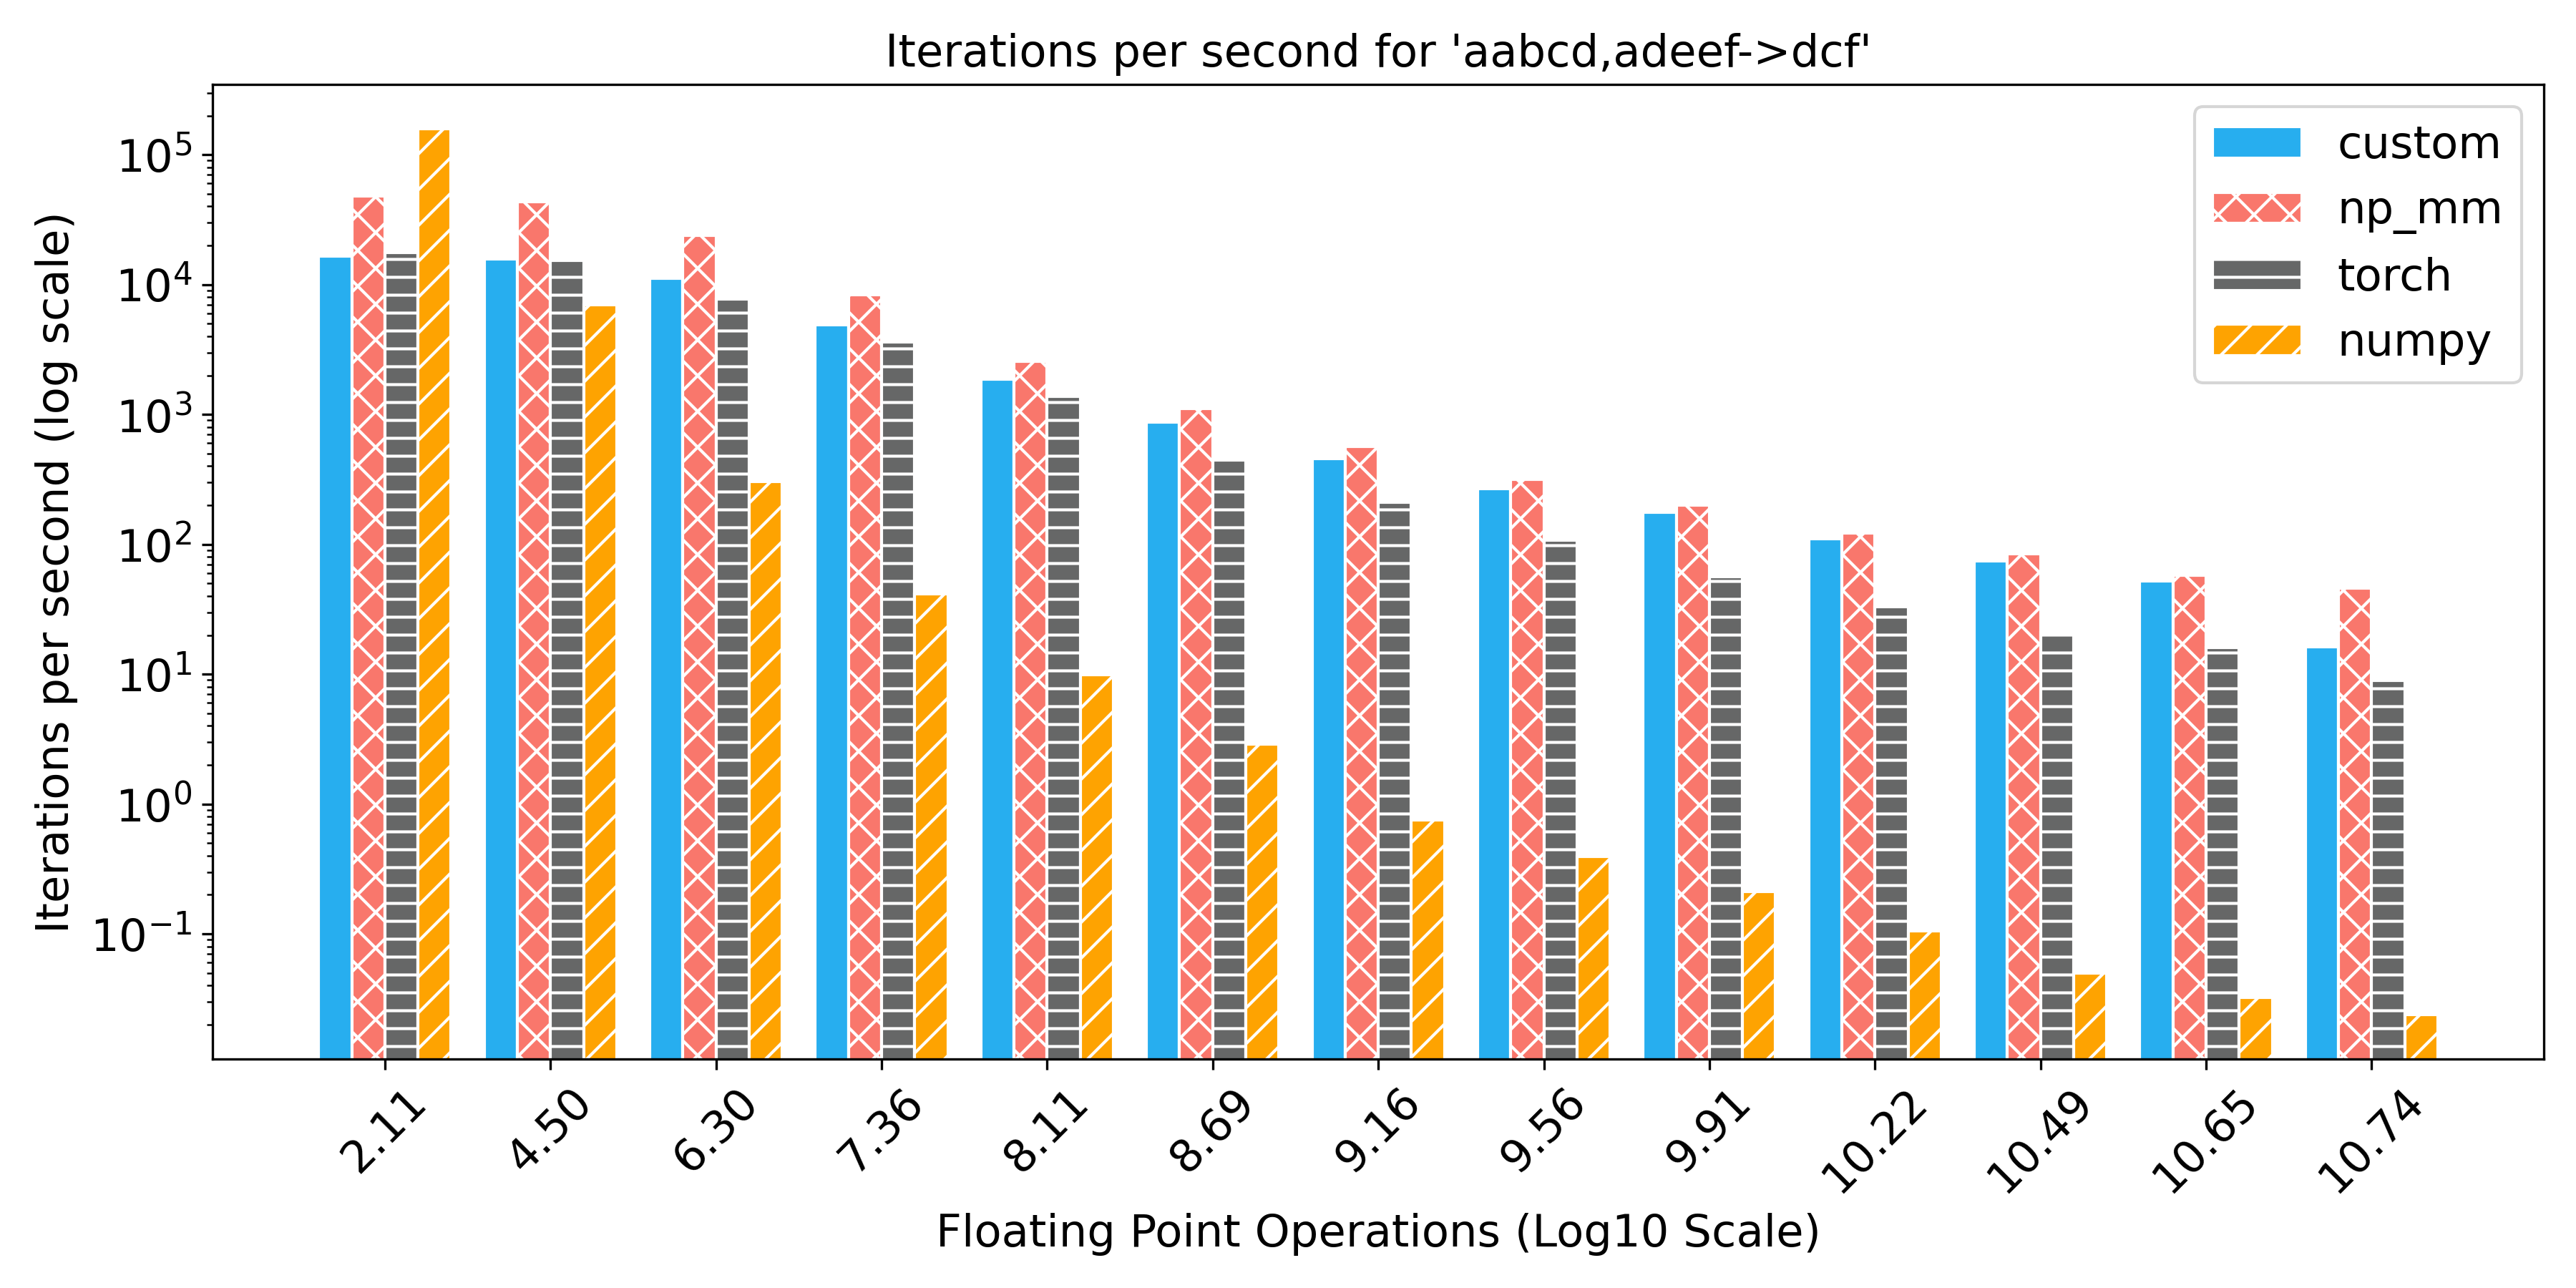
\includegraphics[width=0.49\textwidth]{images/aabcd_adeef__dcf.png} 
    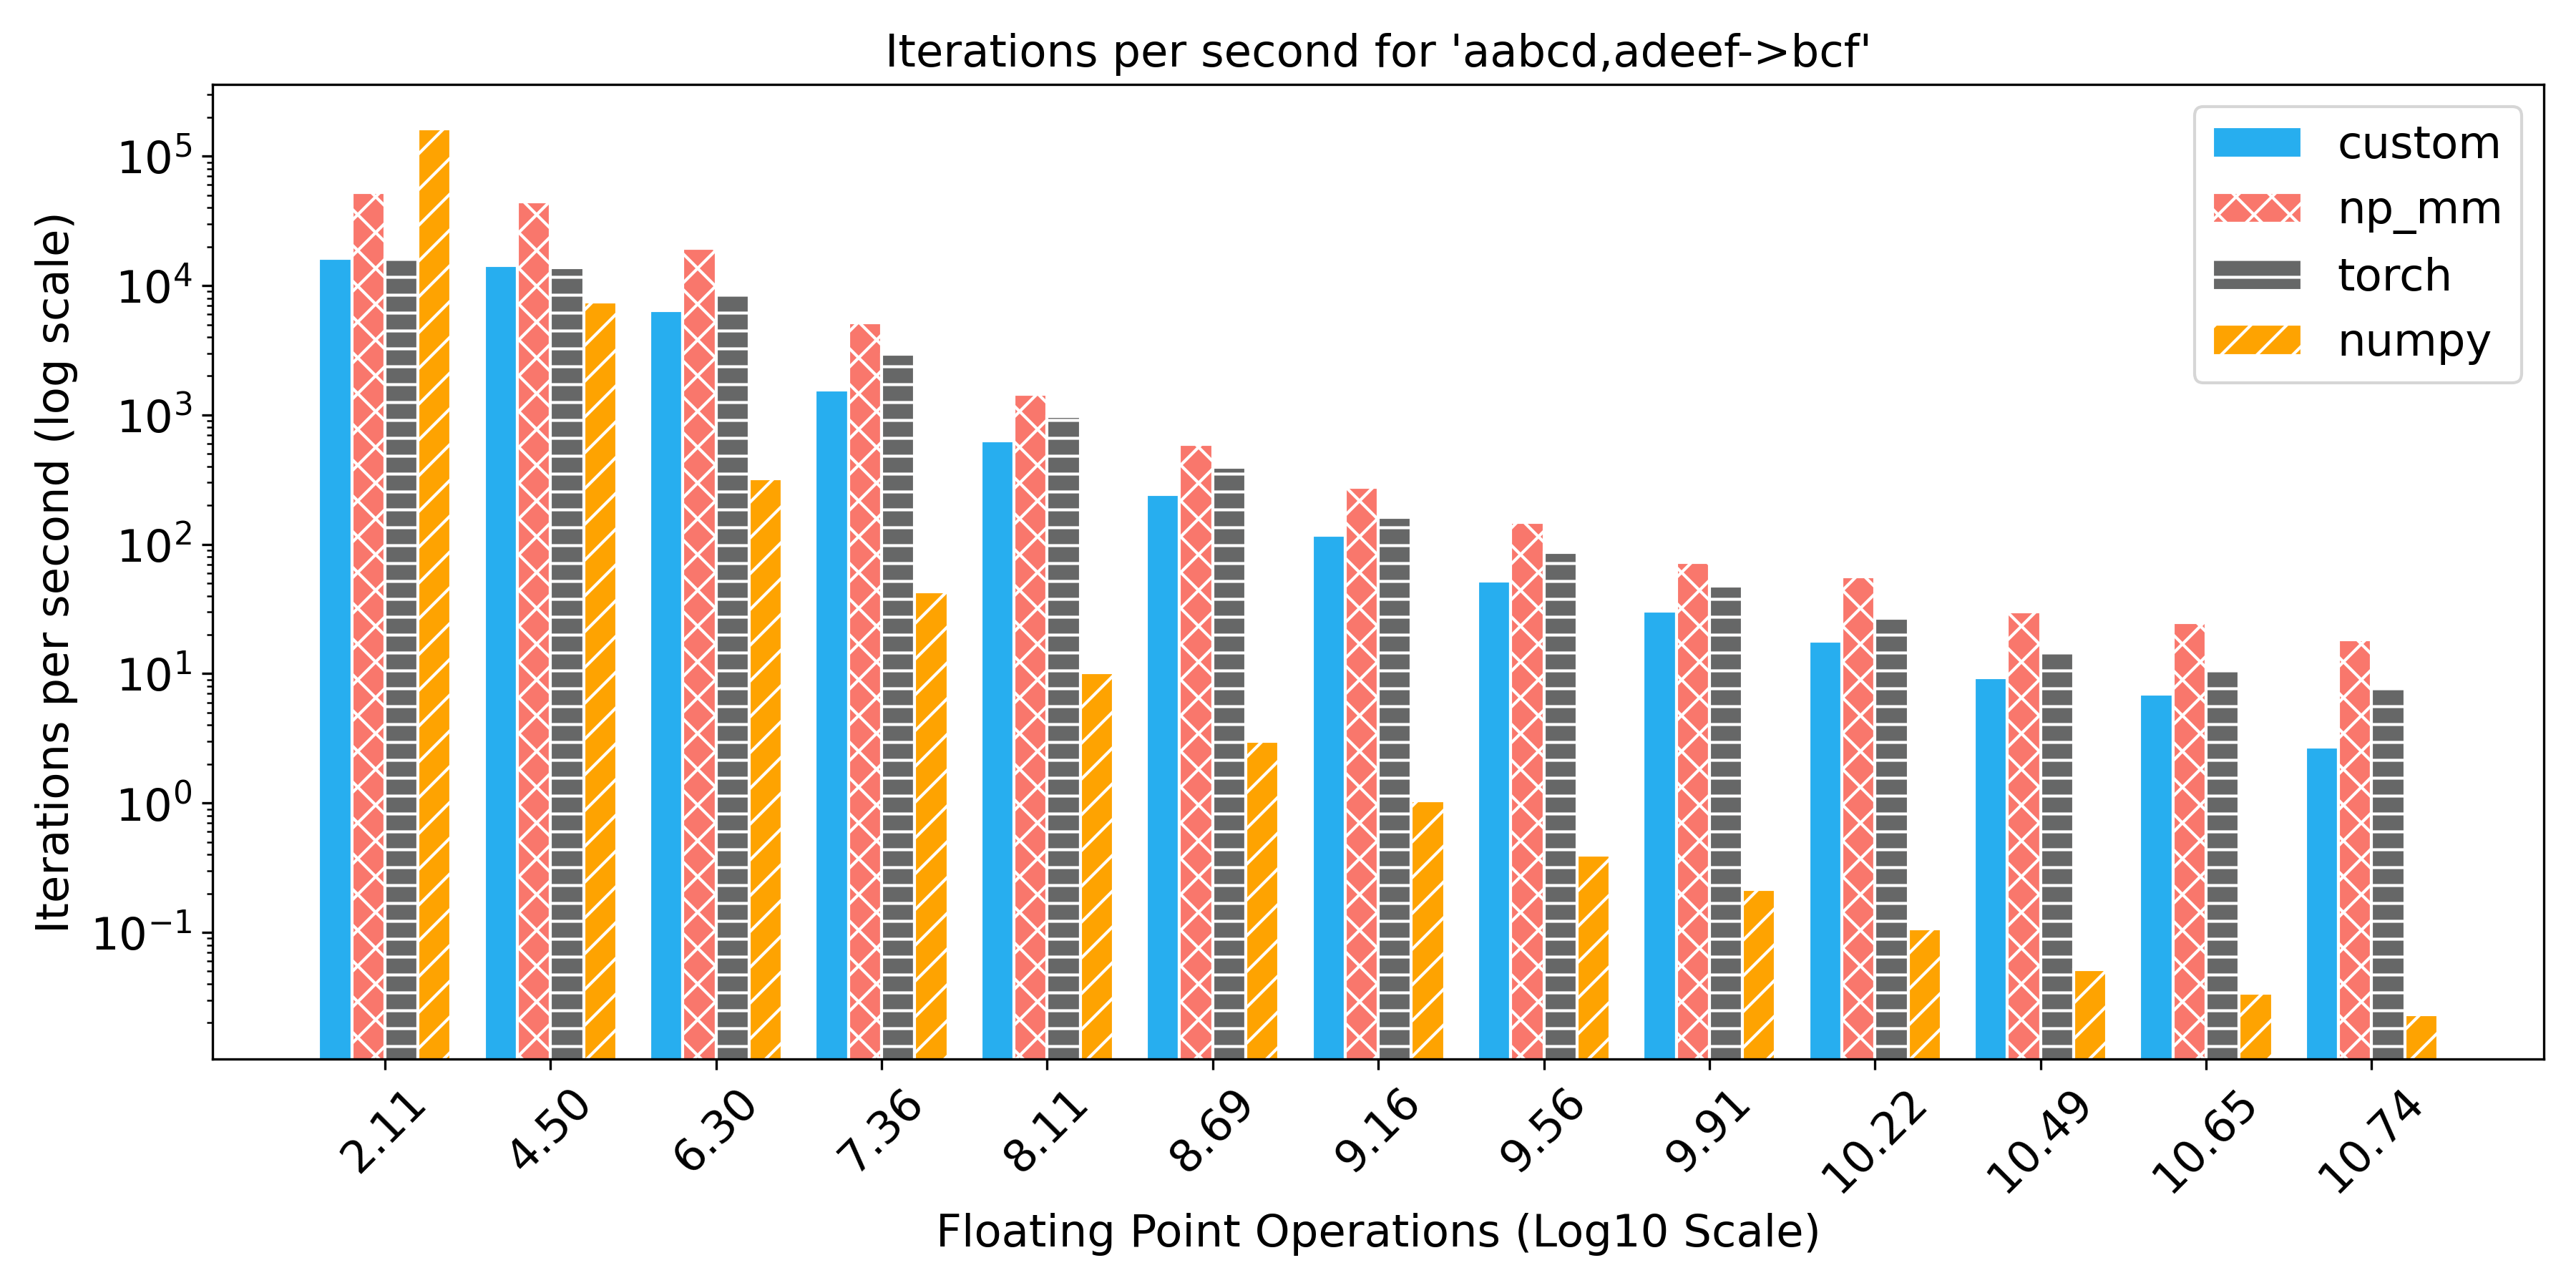
\includegraphics[width=0.49\textwidth]{images/aabcd_adeef__bcf.png} \\
    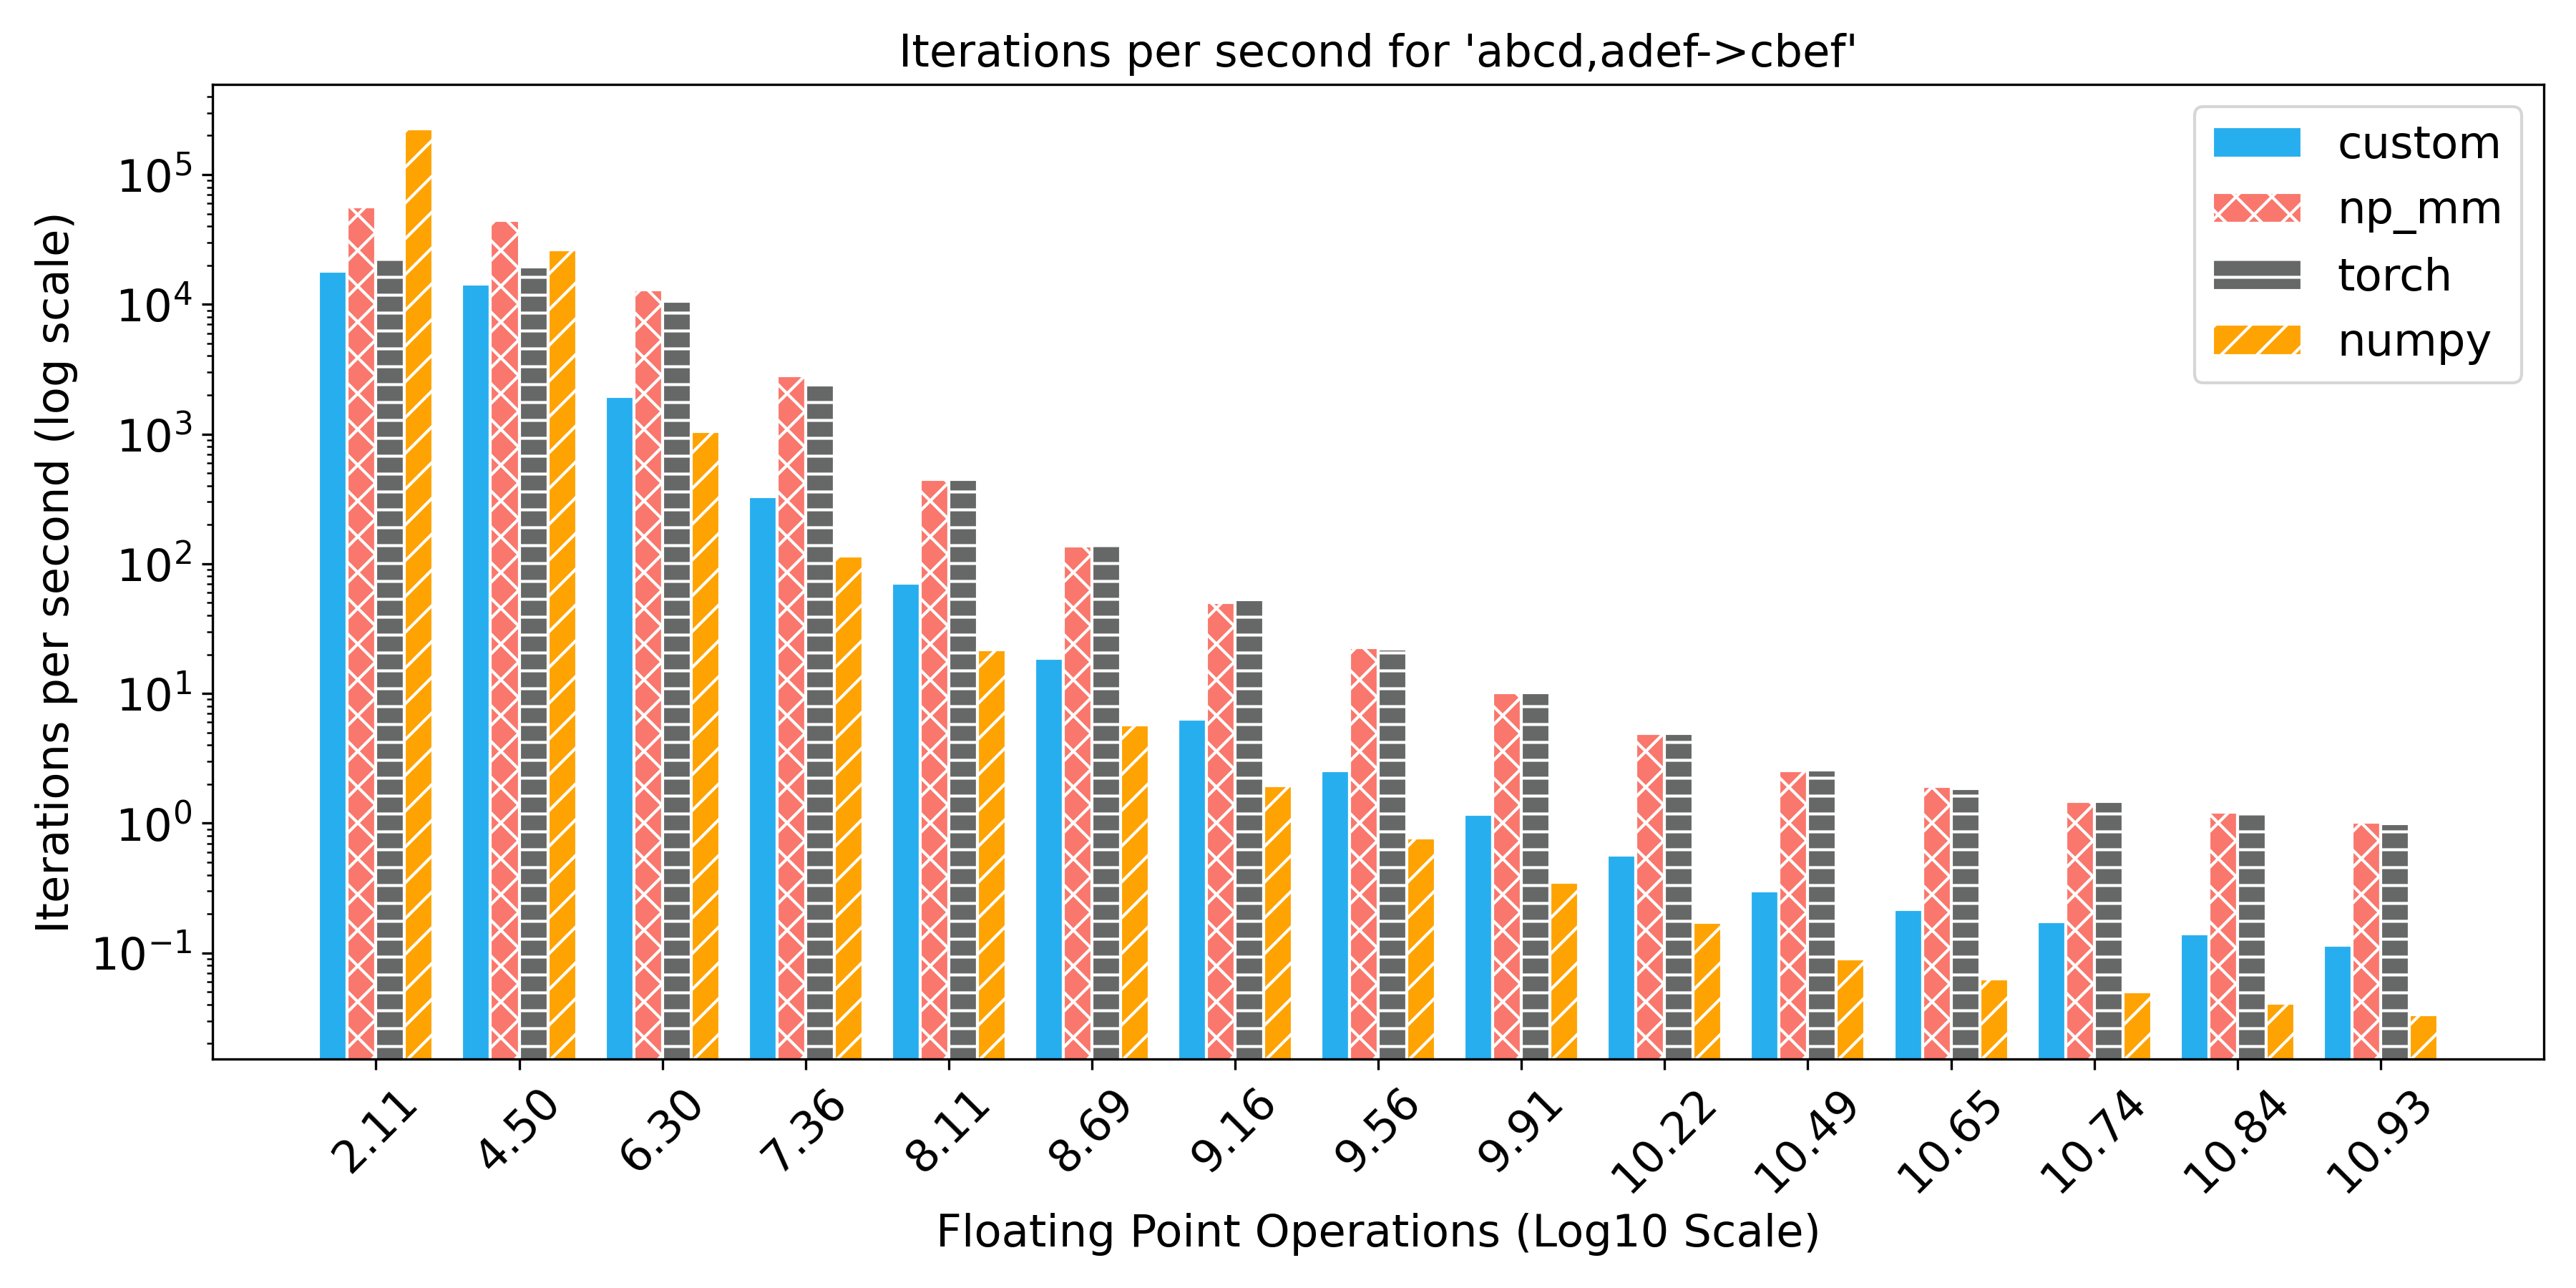
\includegraphics[width=0.49\textwidth]{images/abcd_adef__cbef.png}
    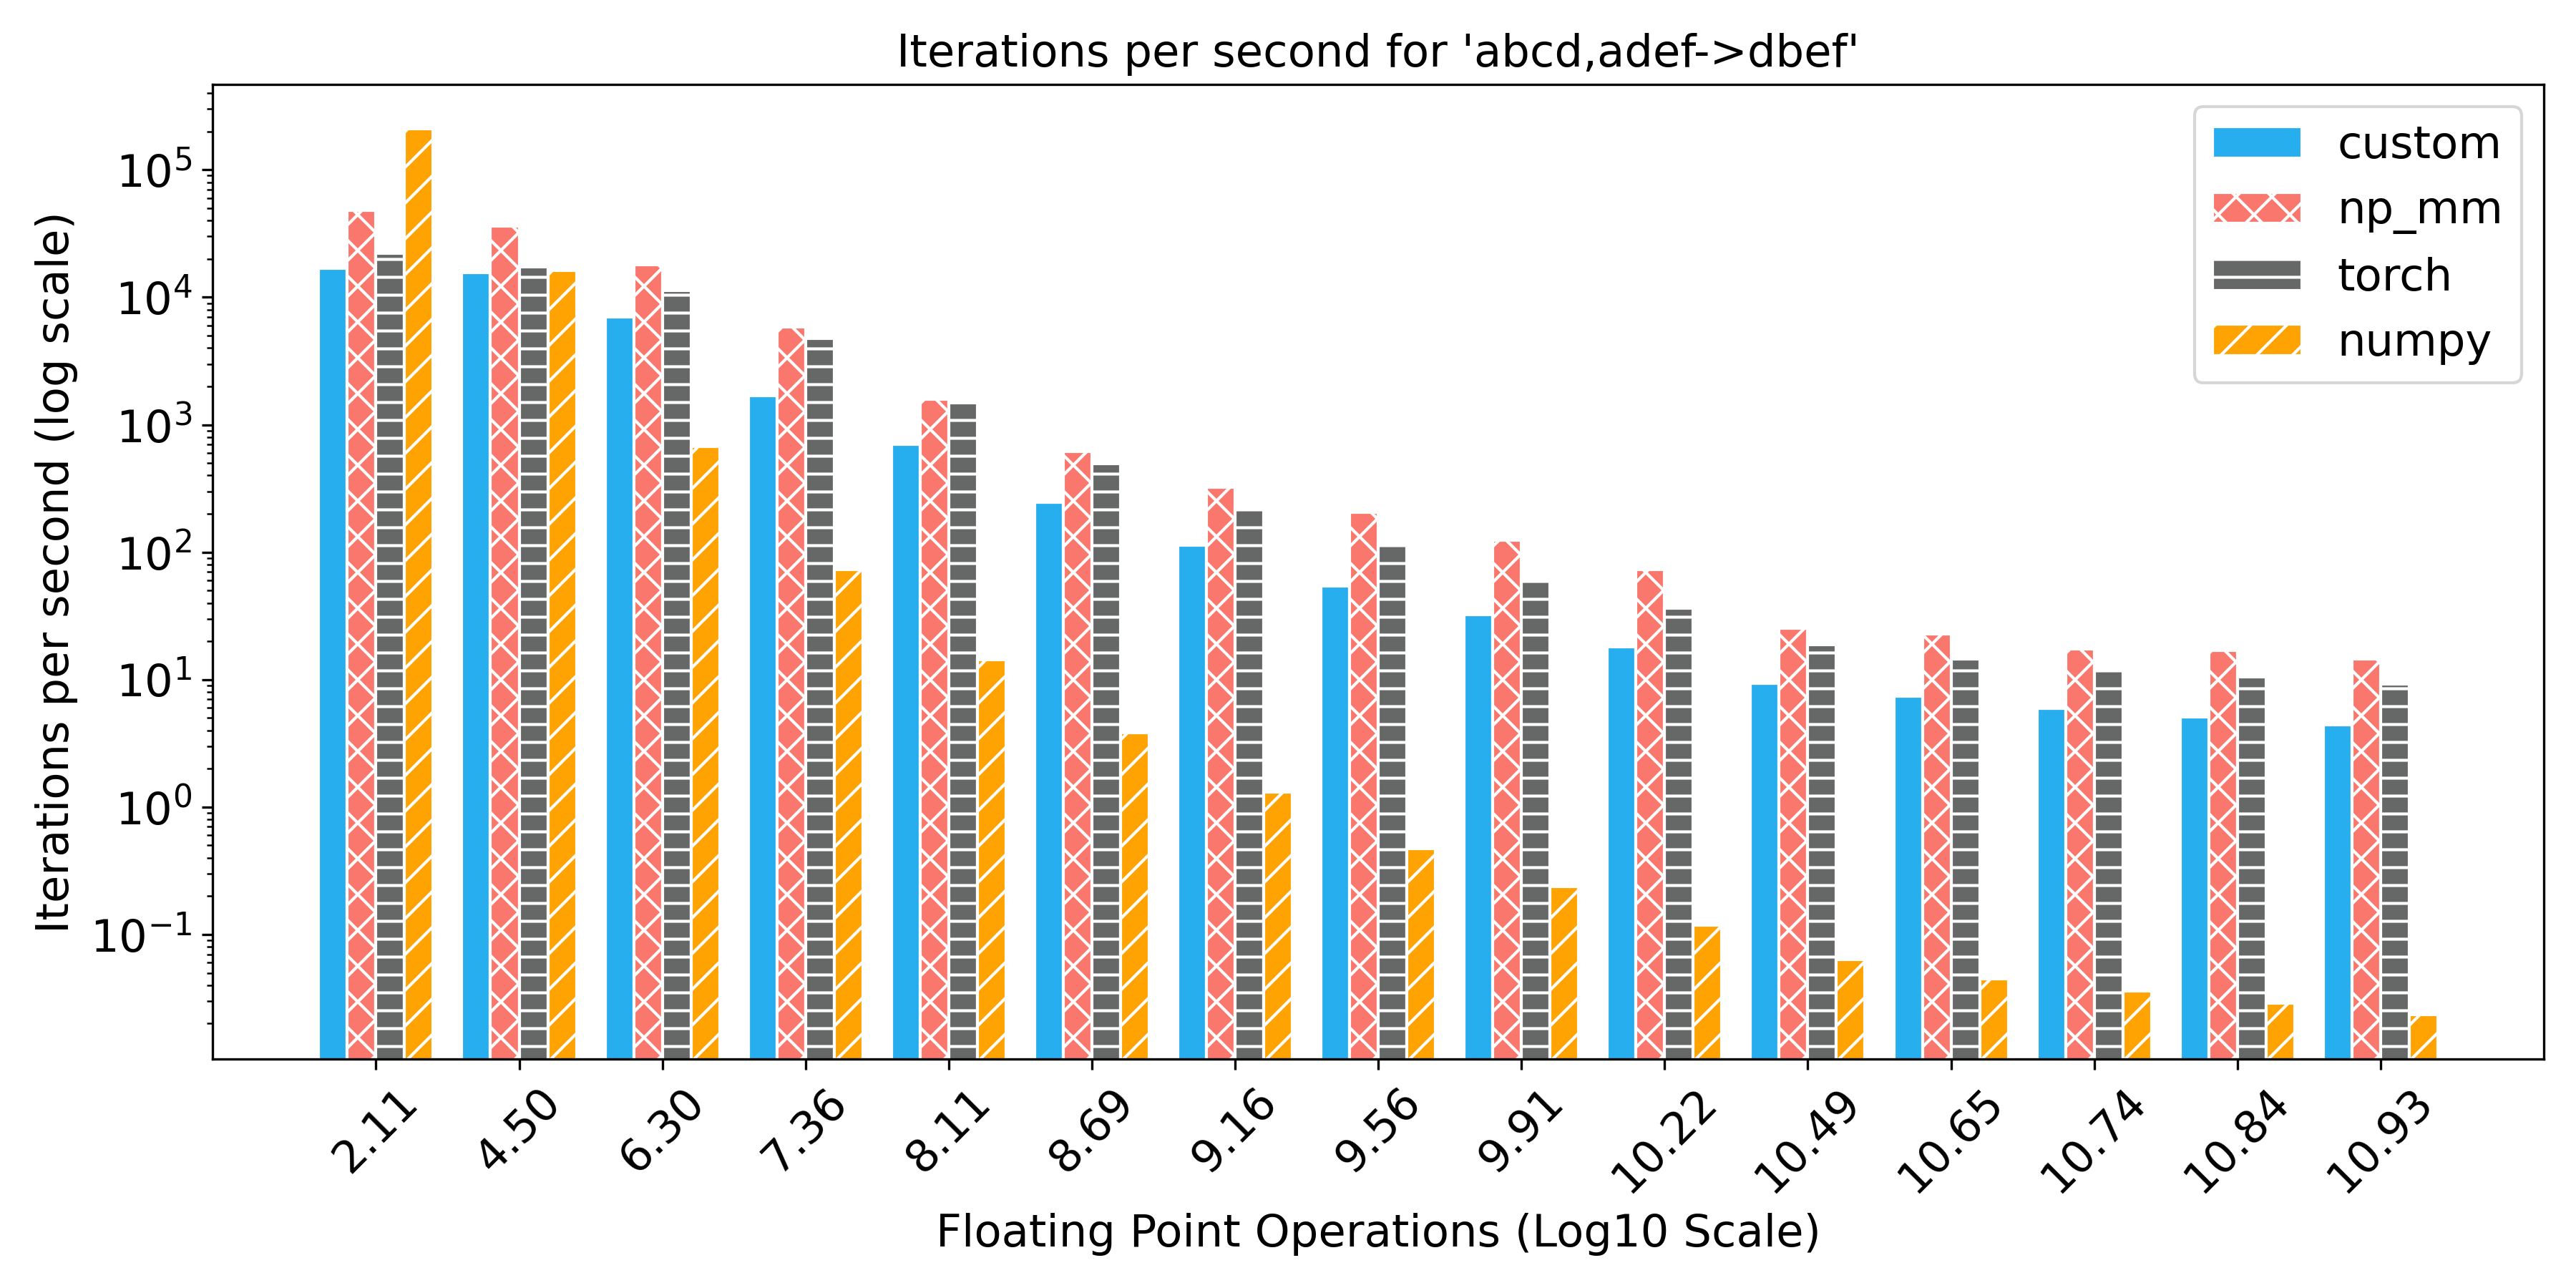
\includegraphics[width=0.49\textwidth]{images/abcd_adef__dbef.png}
    % Include your image
    
\end{figure}

\begin{figure}[H]
    \caption{Performance Comparison for different problems from einsum\_benchmark~\cite{blacher2024einsum}, all tensors casted to float\_64.}
    \label{figure_double}
    \centering
    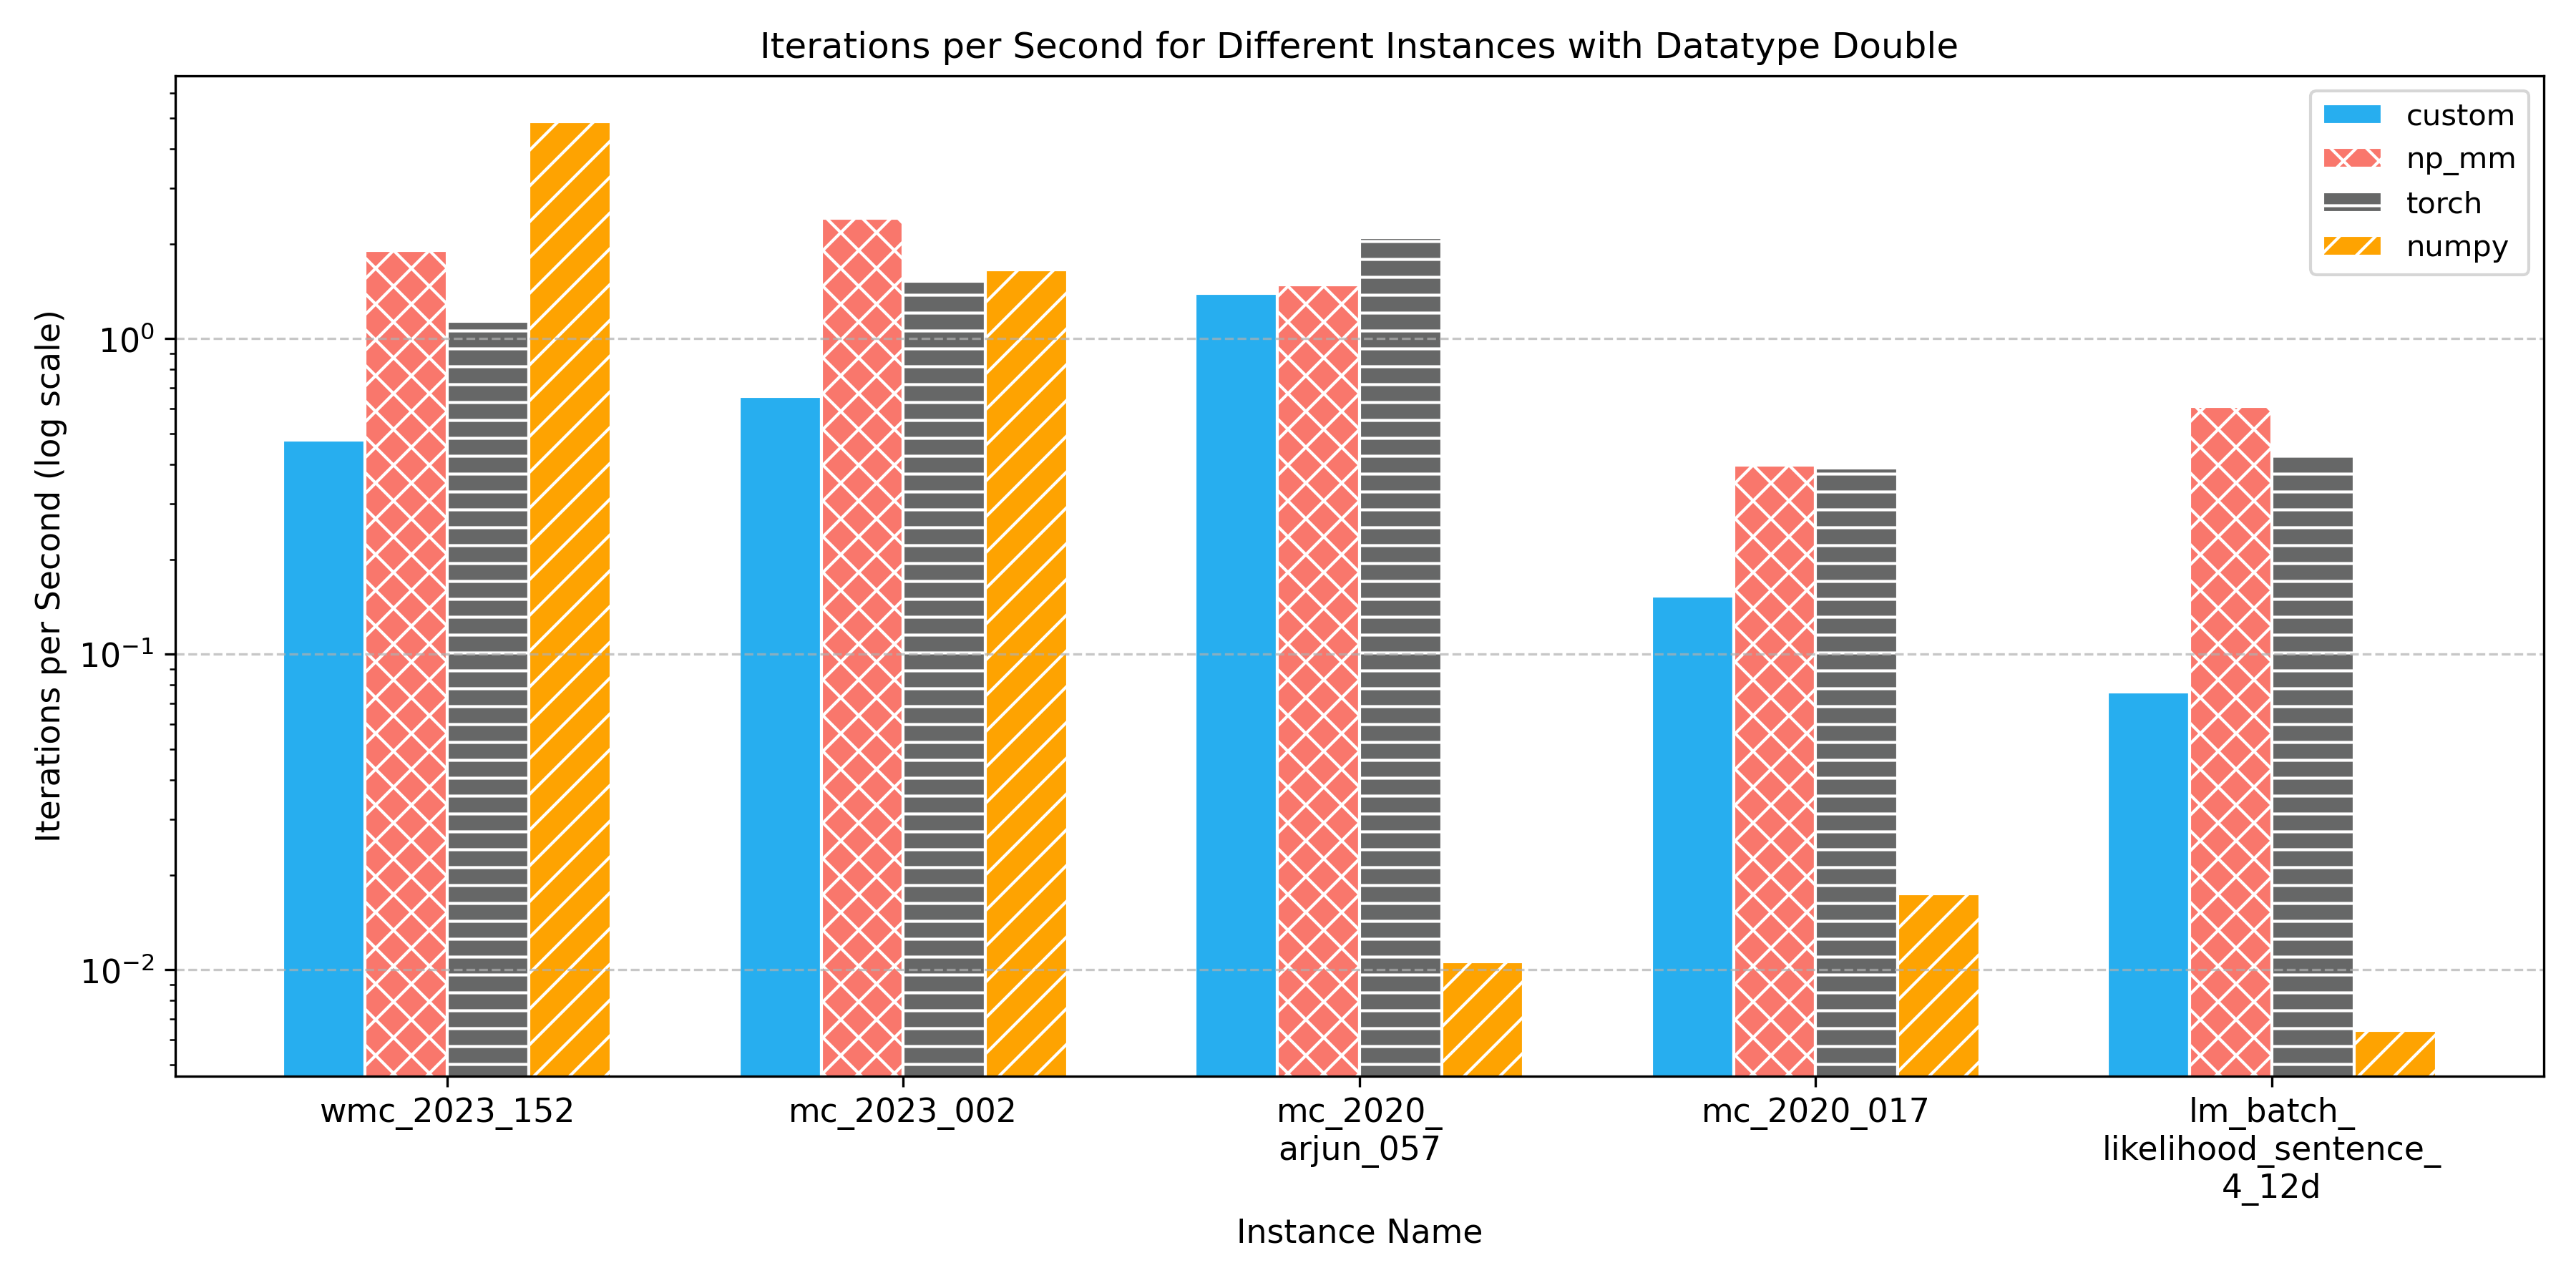
\includegraphics[width=0.75\textwidth]{images/Datatype_Double.png}  % Include your image
    
\end{figure}

%\newgeometry{top=3.0cm, bottom=3.0cm, left=4cm, right=2cm}

\begin{table}[H]
    \caption{Instance data with instance name, number of tensors, and the size of the biggest intermediate tensor.}
    \label{tab:all_properties}
    \centering
    {\tiny
    \begin{tabularx}{\textwidth}{>
    {\raggedright\arraybackslash}p{4cm} >
    {\centering\arraybackslash}X >
    {\centering\arraybackslash}X >
    {\centering\arraybackslash}X}
        \toprule
        \textbf{\tiny Instance Name} & \textbf{\tiny Number of Tensors} & \textbf{\tiny Biggest Intermediate Tensor} & \textbf{\tiny Data Type} \\
        \midrule
        mc\_2022\_167 & 579972 & 64 & int16 \\
        mc\_2022\_079  & 3893 & 2048 & float64 \\
        wmc\_2021\_130 & 5037 & 4096 & float64 \\
        wmc\_2023\_035 & 9049 & 4096 & float64 \\
        str\_matrix\_chain\_multiplication\_1000 & 1000 & 15621 & float64 \\
        str\_mps\_varying\_inner\_product\_2000 & 2000 & 11191 & float64 \\
        wmc\_2023\_152 & 40489 & 16384 & float64 \\
        str\_mps\_varying\_inner\_product\_200 & 200 & 45847 & float64 \\
        mc\_2023\_002  & 26556 & 131072 & float64 \\
        str\_matrix\_chain\_multiplication\_100 & 100 & 233310 & float64 \\
        lm\_batch\_likelihood\_sentence\_4\_4d & 84 & 486400 & float64 \\
        lm\_batch\_likelihood\_brackets\_4\_4d & 84 & 510976 & float64 \\
        mc\_2023\_188  & 14613 & 524288 & float64 \\
        lm\_batch\_likelihood\_sentence\_3\_12d & 38 & 1900800 & float64 \\
        mc\_2020\_017  & 78784 & 4194304 & int32 \\
        lm\_batch\_likelihood\_sentence\_4\_8d & 84 & 7782400 & float64 \\
        mc\_2023\_arjun\_117  & 6267 & 8388608 & float64 \\
        mc\_2021\_027  & 331 & 8388608 & int16 \\
        mc\_rw\_blasted\_case1\_b14\_even3 & 4093 & 8388608 & float64 \\
        str\_nw\_peps\_closed\_333 & 333 & 4976640 & float64 \\
        wmc\_2023\_141 & 230848 & 16777216 & float64 \\
        mc\_2020\_arjun\_046 & 1045 & 8388608 & int64 \\
        mc\_2020\_arjun\_057 & 905 & 8388608 & int32 \\
        mc\_2021\_arjun\_171 & 1601 & 33554432 & float64 \\
        str\_nw\_mera\_closed\_120 & 120 & 31492800 & float64 \\
        lm\_batch\_likelihood\_sentence\_4\_12d & 84 & 39398400 & float64 \\
        str\_nw\_mera\_open\_26 & 26 & 10103940 & float64 \\
        rnd\_mixed\_08 & 500 & 37044000 & float32 \\
        \bottomrule
    \end{tabularx}
    }
\end{table}

\begin{table}[H]
    \caption{Iterations per second for the custom, np\_mm, numpy, and torch over all used problems from einsum\_benchmark~\cite{blacher2024einsum}. The best value in each row is bolded. If a backend failed during the computation due to data type issues, the field is marked with ``-''.}
    \label{tab:all_performance}
    \centering
    {\tiny
    \begin{tabularx}{\textwidth}{%
      >{\raggedright\arraybackslash}p{4cm} %
      >{\centering\arraybackslash}X %
      >{\centering\arraybackslash}X %
      >{\centering\arraybackslash}X %
      >{\centering\arraybackslash}X%
    }
        \toprule
        \textbf{Instance Name} & \textbf{custom} & \textbf{np\_mm} & \textbf{numpy} & \textbf{torch} \\
        \midrule
        mc\_2022\_167 & 0.02902 & 0.10977 & \textbf{0.41380} & – \\
        mc\_2022\_079 & 4.13003 & 12.94602 & \textbf{15.63522} & 8.77809 \\
        wmc\_2021\_130 & 3.07690 & 11.28056 & \textbf{38.19010} & 8.04783 \\
        wmc\_2023\_035 & 1.66732 & 5.58773  & \textbf{9.18394}  & 4.07645 \\
        str\_matrix\_chain\_multiplication\_1000 & 7.57826 & \textbf{25.66862} & 15.57929 & 18.37777 \\
        str\_mps\_varying\_inner\_product\_2000 & 2.98214 & \textbf{9.09908}  & 3.15003  & 6.45833 \\
        wmc\_2023\_152 & 0.46924 & 1.84391  & \textbf{4.88169}  & 1.11984 \\
        str\_mps\_varying\_inner\_product\_200 & 9.01819 & 26.01232 & 7.22079  & \textbf{28.34449} \\
        mc\_2023\_002 & 0.65240 & \textbf{2.21285}  & 1.63918  & 1.46946 \\
        str\_matrix\_chain\_multiplication\_100 & 12.67161 & 37.94583 & 13.49679 & \textbf{53.26709} \\
        lm\_batch\_likelihood\_sentence\_4\_4d & 6.31155 & 10.55606 & 4.68459  & \textbf{12.42889} \\
        lm\_batch\_likelihood\_brackets\_4\_4d & 7.63325 & 12.20857 & 1.40967  & \textbf{13.37427} \\
        mc\_2023\_188 & 0.36408 & 0.76063  & 0.06197  & \textbf{0.91138} \\
        lm\_batch\_likelihood\_sentence\_3\_12d & 3.39126 & \textbf{8.55636}  & 1.25902  & 4.51546 \\
        mc\_2020\_017 & \textbf{0.14763} & 0.14713  & 0.01745  & – \\
        lm\_batch\_likelihood\_sentence\_4\_8d & 0.56249 & \textbf{1.51651}  & 0.17023  & 1.19566 \\
        mc\_2023\_arjun\_117 & 0.26414 & 0.49903  & 0.00457  & \textbf{0.77977} \\
        mc\_2021\_027 & \textbf{3.24499} & 1.81888  & 0.05703  & 2.74746 \\
        mc\_rw\_blasted\_case1\_b14\_even3 & 0.11344 & 0.15607  & 0.02301  & \textbf{0.27253} \\
        str\_nw\_peps\_closed\_333 & 0.30381 & 1.08955  & 0.01631  & \textbf{1.32083} \\
        wmc\_2023\_141 & 0.03194 & 0.06141  & 0.00203  & \textbf{0.06274} \\
        mc\_2020\_arjun\_046 & \textbf{0.42095} & 0.33647  & 0.01436  & 0.30052 \\
        mc\_2020\_arjun\_057 & \textbf{1.26268} & 0.57259  & 0.01066  & 0.70053 \\
        mc\_2021\_arjun\_171 & 0.12230 & 0.13108  & 0.01238  & \textbf{0.24522} \\
        str\_nw\_mera\_closed\_120 & 0.18247 & \textbf{0.96197}  & 0.01679  & 0.87889 \\
        lm\_batch\_likelihood\_sentence\_4\_12d & 0.06761 & \textbf{0.32923}  & 0.00598  & 0.24474 \\
        str\_nw\_mera\_open\_26 & 0.27014 & \textbf{1.49597}  & 0.03690  & 1.39167 \\
        rnd\_mixed\_08 & 0.13898 & 0.24311  & 0.00552  & \textbf{0.38247} \\
        \bottomrule
    \end{tabularx}
    }
\end{table}


\endgroup
